\documentclass{article}
\usepackage{graphicx} % Required for inserting images
\usepackage{subcaption}

\title{Mass Spectroscopy on Gases and simple Organic Molecules \\
Advanced Physics Laboratory}
\author{Fynn Kanja 3780065 \\
Valentino D’Agosto 3763229 \\
Gruppe O43
}


\date{Experiment conducted on: 28. April 2026}



\setlength{\parindent}{0pt}
\setlength{\parskip}{0.5em}
\usepackage[
    backend=biber,
    style=numeric,
  ]{biblatex}

 \addbibresource{quellen.bib}



\begin{document}

\begin{figure}
    \centering
    
\includegraphics[width=0.75\linewidth]{uni_logo.png}
\end{figure}

\maketitle


\begin{abstract}

\end{abstract}
\newpage
\begingroup
\tableofcontents
\endgroup
%\listoffigures
%\listoftables

\newpage



\section{Introduction}
\subsection{Theoretical Overview}

\subsubsection{Massendefekt}

Eine wichtige Konsequenz der unterschiedlichen Neutronenzahl bei Isotopen ist ein Phänomen, das als Massendefekt bezeichnet wird. Aufgrund der anziehenden Kernkräfte ist Energie erforderlich, um einen Atomkern in seine einzelnen Nukleonen zu zerlegen. Diese Energie wird als gesamte Bindungsenergie $E_B$ definiert. Die mittlere Bindungsenergie pro Nukleon ergibt sich dann zu $\bar{E}_B = E_B/A$, wobei $A$ die Massenzahl bezeichnet.

Legt man das Minimum der potentiellen Energie auf den Zustand der vollständig voneinander getrennten Nukleonen fest, so erhält man für das System des zusammengesetzten Kerns eine negative Energie. Gemäß der Einstein'schen Beziehung $E = mc^2$ entspricht diese negative Bindungsenergie $-E_B$ einem Massendefekt
\begin{equation}
    \Delta M = \frac{E_B}{c^2}
\end{equation}
des Kerns gegenüber der Summe der Massen aller seiner Nukleonen. Folglich ist die Masse des Atomkerns um den Betrag $\Delta M$ kleiner als die Summe der Massen aller in ihm enthaltenen Protonen und Neutronen.


\subsubsection{Mittlere freie Weglänge}
Die mittlere freie Weglänge beschreibt die Strecke, die ein Teilchen in einem gegebenen Material zurücklegen kann, bevor es auf irgendeine Weise mit einem anderen Teilchen zusammenstößt. Zur Bestimmung der mittleren freien Weglänge betrachten wir zunächst ein vereinfachtes Modell, in dem alle übrigen Teilchen als ruhend angenommen werden. Diese Annahme ist gerechtfertigt, da bei einer Ionengeschwindigkeit, die einer Energie von $1\,\mathrm{eV}$ entspricht, die äquivalente Gastemperatur in der Größenordnung von $4 \cdot 10^4\,\mathrm{K}$ liegt \cite{Frieser1979}.
Ein Stoß findet statt, wenn der Abstand zwischen zwei Teilchen kleiner als der Teilchendurchmesser $d$ ist. Dies definiert einen effektiven Stoßquerschnitt
\begin{equation}
    \sigma = \pi d^2.
\end{equation}
Das bewegte Teilchen überstreicht entlang seiner Bahn ein Volumen, welches als Zylinder mit dem Querschnitt $\sigma$ interpretiert werden kann. Für eine Weglänge $\ell$ ergibt sich das überstrichene Volumen zu
\begin{equation}
    V = \pi d^2 \ell.
\end{equation}
Mit der Teilchenzahldichte $N_v$ ergibt sich die Anzahl der Stöße in diesem Volumen zu
\begin{equation}
    N = N_v \, V = N_v \pi d^2 \ell.
\end{equation}
Die mittlere freie Weglänge $\Lambda_{Ion}$ erhält man, indem man $N = 1$ setzt, woraus
\begin{equation}
    \Lambda_{Ion} = \frac{1}{\pi d^2 N_v}
    \label{eq:mean_free_path_simple}
\end{equation}
folgt. Eine genauere Beschreibung der mittleren freien Weglänge berücksichtigt die Maxwell'sche Geschwindigkeitsverteilung der Gasteilchen. In diesem Fall verringert sich die mittlere freie Weglänge um einen Faktor $\sqrt{2}$ \cite{WikiMFP}, sodass sich
\begin{equation}
    \Lambda_{Ion} = \frac{1}{\sqrt{2}\,\pi d^2 N_v}
    \label{eq:mean_free_path_maxwell}
\end{equation}
ergibt.


\subsubsection{Ionisierungspotential}
Das Ionisierungspotential (auch Ionisierungsenergie genannt) bezeichnet die minimale Energie, die benötigt wird, um ein Elektron aus einem neutralen Atom oder Molekül im Grundzustand vollständig zu entfernen und so ein einfach positiv geladenes Ion zu erzeugen:
\begin{equation}
    A + E_i \rightarrow A^+ + e^-.
\end{equation}
Die Ionisierungsenergie wird üblicherweise in Elektronenvolt ($\mathrm{eV}$) angegeben und hängt von der Elektronenkonfiguration des jeweiligen Atoms ab. Edelgase weisen aufgrund ihrer abgeschlossenen Elektronenschalen besonders hohe Ionisierungsenergien auf, während Alkalimetalle nur ein schwach gebundenes Valenzelektron besitzen und entsprechend niedrige Werte aufweisen. Für die Erzeugung mehrfach geladener Ionen sind die zweite, dritte usw.\ Ionisierungsenergien erforderlich, welche aufgrund der stärkeren Bindung der verbleibenden Elektronen sukzessive größer werden. In der Massenspektrometrie ist die Kenntnis des Ionisierungspotentials von Bedeutung, da die Energie der ionisierenden Elektronen in der Ionenquelle ausreichend hoch sein muss, um die Probenmoleküle effizient zu ionisieren.

\subsubsection{Isotopenmuster}
Die meisten chemischen Elemente kommen in der Natur als Gemisch verschiedener Isotope vor, die sich in der Anzahl der Neutronen im Atomkern unterscheiden, bei identischer Protonenzahl. Da Isotope eines Elements nahezu dieselben chemischen Eigenschaften, aber unterschiedliche Massen besitzen, erscheinen sie im Massenspektrum als charakteristisches Muster mehrerer Peaks. Das Verhältnis der Peakhöhen entspricht dabei der natürlichen relativen Häufigkeit der jeweiligen Isotope. So besitzt beispielsweise Krypton sechs stabile Isotope mit den Massenzahlen 78, 80, 82, 83, 84 und 86, wobei $^{84}\mathrm{Kr}$ mit etwa $57\,\%$ die größte Häufigkeit aufweist. Das Isotopenmuster dient in der Massenspektrometrie als wichtiges Werkzeug zur Identifikation von Elementen und Molekülen, da es einen charakteristischen ,,Fingerabdruck`` darstellt. Bei Molekülen ergibt sich das beobachtete Muster aus der Faltung der Isotopenverteilungen aller im Molekül enthaltenen Elemente.

\subsubsection{Fragmentierung}
Bei der Ionisierung in der Ionenquelle wird den Molekülen häufig deutlich mehr Energie zugeführt, als für die reine Ionisierung notwendig wäre. Diese überschüssige Energie kann zum Aufbrechen chemischer Bindungen innerhalb des Moleküls führen, was als Fragmentierung bezeichnet wird. Aus einem Molekülion $M^+$ entstehen dabei kleinere geladene Bruchstücke (Fragment-Ionen) sowie neutrale Teilchen, die im Massenspektrometer nicht detektiert werden. Im Massenspektrum erscheint neben dem sogenannten Molekülpeak (auch Hauptpeak oder ,,parent peak``), der dem unfragmentierten Molekülion entspricht, eine Reihe weiterer Peaks bei kleineren Masse-zu-Ladungs-Verhältnissen, die den verschiedenen Fragment-Ionen zuzuordnen sind. Das resultierende Fragmentierungsmuster ist für jede Molekülsorte charakteristisch und kann mit Referenzspektren aus Datenbanken verglichen werden, wodurch eine eindeutige Identifikation auch unbekannter Substanzen ermöglicht wird. Die Fragmentierung liefert somit wertvolle Informationen über die Struktur des untersuchten Moleküls.



\subsection{Experimenteller Aufbau}
Der allgemeine Aufbau eines Massenspektrometers besteht aus drei Komponenten. Die \textbf{Ionenquelle}, in der die Probe in einen gasförmigen Zustand überführt und ionisiert wird, meist durch das Entfernen eines Elektrons. Der \textbf{Analysator}, der in unserem Fall ein Quadrupol-Massenspektrometer (\textbf{QMS}) ist und für die Trennung der Atome nach ihrem Masse-zu-Ladungs-Verhältnis ($\frac{m}{q}$) verantwortlich ist, was häufig mithilfe eines magnetischen und elektrischen Feldes erfolgt. Und der \textbf{Detektor}, der die eintreffenden Teilchen registriert und in ein elektrisches Signal umwandelt, mit dem weiter gearbeitet werden kann. \label{core_comp_mass_spctrmtr}


\subsubsection{Setup of the QMS}
\textbf{! TODO !}

\subsubsection{Funktionsweise des QMS}
\begin{figure}
    \centering
    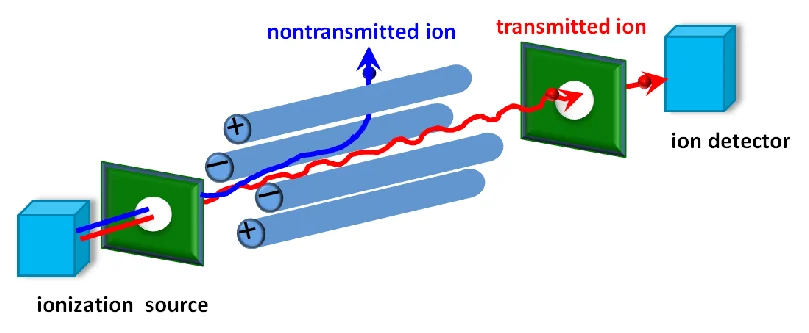
\includegraphics[width=1\linewidth]{QMS_schematic.png}
    \caption{Schematische Darstellung des Quadrupol-Massenspektrometers mit den Kernkomponenten, die in Kapitel \ref{core_comp_mass_spctrmtr} erläutert werden, sowie dem Funktionsprinzip eines QMS.}
    %Source: https://www.researchgate.net/figure/Scheme-of-quadrupole-mass-analyzer-Q_fig4_329040300
    \label{fig:qms_schematic}
\end{figure}
Das Quadrupol-Massenspektrometer besitzt als Analysator einen Quadrupol, der aus vier präzise gefertigten, runden Stäben aus Edelstahl oder Molybdän besteht. Diese Pole sind parallel im Abstand $r$ um die Symmetrieachse angeordnet. Die gegenüberliegenden Stäbe liegen jeweils auf dem gleichen Potential. An den benachbarten Stäben liegt eine Gleichspannung ($U$) sowie eine Wechselspannung mit der Amplitude $V$ an:
\begin{equation}
    u(t) = U + V \cos(\omega t).
\end{equation}
Die Bahnen der Ionen im Inneren des Quadrupol-Massenspektrometers lassen sich durch die Mathieu'sche Differentialgleichung beschreiben:
\begin{equation}
    \frac{d^2 y}{dx^2} + (a - 2q \cos(2\xi))\, y = 0.
\end{equation}
Die Lösungen dieser Differentialgleichung weisen bekanntermaßen sowohl stabile als auch instabile Bahnen auf. Über die Parameter Frequenz $\omega$ und die Spannungen $U$ und $V$ lässt sich einstellen, welche Ionen mit dem passenden Masse-zu-Ladungs-Verhältnis den Detektor auf einer zentralen Trajektorie erreichen können. Die Bahn der Teilchen mit dem richtigen $\frac{m}{q}$-Verhältnis verläuft sinusförmig mit gleichen Abständen der Amplituden zur Symmetrieachse des Quadrupols. Teilchen mit einem abweichenden Verhältnis folgen zwar ebenfalls einer sinusförmigen Bahn, werden jedoch zunehmend aus dem Quadrupol heraus beschleunigt, bis sie das elektromagnetische Feld verlassen. Auf diese Weise erreichen nur Teilchen mit dem passenden Verhältnis den Detektor am Ende des Massenspektrometers.
\cite{Wiki_Quadrupol} \cite{Wiki_Mathiu_func}



\section{Aufgabe 1}


\section{Aufgabe 2}
\section{Aufgabe 3}
\section{Aufgabe 4}
\section{Aufgabe 5}



\newpage
\printbibliography %[heading=none]

\end{document}
